% **************************************************
% Document Class Definition
% **************************************************
\documentclass[%
	paper=A4,					% paper size --> A4 is default in Germany
	twoside=true,				% onesite or twoside printing
	openright,					% doublepage cleaning ends up right side
	parskip=full,				% spacing value / method for paragraphs
	chapterprefix=true,			% prefix for chapter marks
	11pt,						% font size
	headings=normal,			% size of headings
	bibliography=totoc,			% include bib in toc
	listof=totoc,				% include listof entries in toc
	titlepage=on,				% own page for each title page
	captions=tableabove,		% display table captions above the float env
	draft=false,				% value for draft version
]{scrreprt}%

% **************************************************
% Debug LaTeX Information
% **************************************************
%\listfiles

% **************************************************
% Information and Commands for Reuse
% **************************************************
\newcommand{\ie}{\textit{i.e.,}\xspace}
\newcommand{\eg}{\textit{e.g.,}\xspace}
\newcommand{\etc}{\textit{etc.}\xspace}
\newcommand{\thesisTitle}{Generaci�n autom�tica de tests para aplicaciones Android basada en multi-modelos}
\newcommand{\thesisName}{Mar�a Isabel Ar�valo Robinson}
\newcommand{\thesisSubject}{Proyecto de grado}
\newcommand{\thesisDate}{Diciembre, 2018}
\newcommand{\thesisVersion}{1.0}

\newcommand{\thesisFirstReviewer}{Ph.D. Nicol\'{a}s Cardozo }
\newcommand{\thesisFirstReviewerUniversity}{\protect{Universidad de los Andes, Bogot\'{a}, Colombia}}
\newcommand{\thesisFirstReviewerDepartment}{Departamento de Ingenier�a de Sistemas y Computaci�n}

\newcommand{\thesisSecondReviewer}{Ph.D. Gabriele Bavota}
\newcommand{\thesisSecondReviewerUniversity}{\protect{Universit\`{a} della Svizzera italiana (USI), Lugano}}
\newcommand{\thesisSecondReviewerDepartment}{Faculty of Informatics }

\newcommand{\thesisFirstSupervisor}{Ph.D. Mario Linares V\'{a}squez}

\newcommand{\thesisUniversity}{\protect{Universidad de los Andes}}
\newcommand{\thesisUniversityDepartment}{Departamento de Ingenier�a de Sistemas y Computaci�n}
\newcommand{\thesisUniversityInstitute}{Facultad de Ingenier�a}
\newcommand{\thesisUniversityGroup}{The Software Design Lab}
\newcommand{\thesisUniversityCity}{Bogot\'{a}, Colombia}
\newcommand{\thesisUniversityStreetAddress}{Cra 1 \# 18A - 12}
\newcommand{\thesisUniversityPostalCode}{111711}



% **************************************************
% Load and Configure Packages
% **************************************************
\usepackage[T1]{fontenc}
\usepackage[utf8]{inputenc}		% defines file's character encoding
\usepackage[spanish]{babel} % babel system, adjust the language of the content
\usepackage[					% clean thesis style
	figuresep=colon,%
	sansserif=false,%
	hangfigurecaption=false,%
	hangsection=true,%
	hangsubsection=true,%
	colorize=full,%
	colortheme=bluemagenta,%
	bibsys=bibtex,%
	bibfile=bib-refs,%
	bibstyle=numeric,%
]{cleanthesis}
\usepackage[linesnumbered]{algorithm2e}
\usepackage{adjustbox}
\usepackage{listings,color}
\usepackage{amsfonts}
\usepackage{tcolorbox}
\usepackage{amssymb}
\usepackage{ifthen}
\lstset{
	language=xml,
	tabsize=2,
	%frame=lines,
	frame=shadowbox,
	rulesepcolor=\color{gray},
	xleftmargin=18pt,
	framexleftmargin=15pt,
	keywordstyle=\color{blue},
	commentstyle=\color{OliveGreen},
	stringstyle=\color[rgb]{0,0.43,0.72},
	numbers=left,
	numberstyle=\tiny,
	numbersep=4pt,
	breaklines=true,
	showstringspaces=false,
	basicstyle=\ttfamily\scriptsize,
	columns=fullflexible,
	emph={node,name,price},emphstyle={\color{magenta}}}

\colorlet{punct}{red!60!black}
\definecolor{background}{HTML}{EEEEEE}
\definecolor{delim}{RGB}{20,105,176}
\colorlet{numb}{magenta!60!black}
\lstdefinelanguage{json}{
	basicstyle=\ttfamily\scriptsize,
	numbers=left,
	numberstyle=\scriptsize,
	stepnumber=1,
	numbersep=8pt,
	showstringspaces=false,
	breaklines=true,
	frame=shadowbox,
	literate=
	*{0}{{{\color{numb}0}}}{1}
	{1}{{{\color{numb}1}}}{1}
	{2}{{{\color{numb}2}}}{1}
	{3}{{{\color{numb}3}}}{1}
	{4}{{{\color{numb}4}}}{1}
	{5}{{{\color{numb}5}}}{1}
	{6}{{{\color{numb}6}}}{1}
	{7}{{{\color{numb}7}}}{1}
	{8}{{{\color{numb}8}}}{1}
	{9}{{{\color{numb}9}}}{1}
	{:}{{{\color{punct}{:}}}}{1}
	{,}{{{\color{punct}{,}}}}{1}
	{\{}{{{\color{delim}{\{}}}}{1}
	{\}}{{{\color{delim}{\}}}}}{1}
	{[}{{{\color{delim}{[}}}}{1}
	{]}{{{\color{delim}{]}}}}{1},
}

\lstloadlanguages{xml}
\renewcommand{\lstlistingname}{Code example}% Listing -> Algorithm
\renewcommand{\lstlistlistingname}{List of \lstlistingname s}


\hypersetup{					% setup the hyperref-package options
	pdftitle={\thesisTitle},	% 	- title (PDF meta)
	pdfsubject={\thesisSubject},% 	- subject (PDF meta)
	pdfauthor={\thesisName},	% 	- author (PDF meta)
	plainpages=false,			% 	-
	colorlinks=false,			% 	- colorize links?
	pdfborder={0 0 0},			% 	-
	breaklinks=true,			% 	- allow line break inside links
	bookmarksnumbered=true,		%
	bookmarksopen=true			%
}

\newcommand{\nb}[2]{
	\fbox{\bfseries\sffamily\scriptsize#1}
	{\small$\blacktriangleright$\textit{#2}$\blacktriangleleft$}}
\newcommand\MARIO[1]{\textcolor{red}{\nb{MARIO}{#1}}}
\newcommand\SANTIAGO[1]{\textcolor{orange}{\nb{SANTIAGO}{#1}}}
% **************************************************
% Document CONTENT
% **************************************************
\begin{document}

% --------------------------
% rename document parts
% --------------------------
%\renewcaptionname{ngerman}{\figurename}{Abb.}
%\renewcaptionname{ngerman}{\tablename}{Tab.}
\renewcaptionname{spanish}{\figurename}{Fig.}
\renewcaptionname{spanish}{\tablename}{Tab.}

% --------------------------
% Front matter
% --------------------------
\pagenumbering{roman}			% roman page numbing (invisible for empty page style)
\pagestyle{empty}				% no header or footers
% !TEX root = ../thesis-example.tex
%
% ------------------------------------  --> cover title page
\begin{titlepage}
	\pdfbookmark[0]{Cover}{Cover}
	\flushright
	\hfill
	\vfill
	{\LARGE\thesisTitle \par}
	\rule[5pt]{\textwidth}{.4pt} \par
	{\Large\thesisName}
	\vfill
	\textit{\large\thesisDate} \\
	Version: \thesisVersion
\end{titlepage}


% ------------------------------------  --> main title page
\begin{titlepage}
	\pdfbookmark[0]{Titlepage}{Titlepage}
	\tgherosfont
	\centering

	Bogotá, Colombia \\[4mm]
	
\includegraphics[width=6cm]{gfx/logo-uniandes} \\[2mm]
	\textsf{\thesisUniversityDepartment} \\
	\textsf{\thesisUniversityInstitute} \\
	\textsf{\thesisUniversityGroup} \\

	\vfill
	{\large \thesisSubject} \\[5mm]
	{\LARGE \color{ctcolortitle}\textbf{\thesisTitle} \\[10mm]}
	{\Large \thesisName} \\

	\vfill
		\begin{minipage}[t]{.27\textwidth}
		\raggedleft
		\textit{Asesor}
	\end{minipage}
	\hspace*{15pt}
	\begin{minipage}[t]{.65\textwidth}
		{\Large \thesisFirstSupervisor} \\
		{\small \thesisFirstReviewerDepartment} \\[-1mm]
		{\small \thesisFirstReviewerUniversity}
	\end{minipage} \\[5mm]

	\thesisDate \\

\end{titlepage}


% ------------------------------------  --> lower title back for single page layout
\hfill
\vfill
{
	\small
	\textbf{\thesisName} \\
	\textit{\thesisTitle} \\
	\thesisSubject, \thesisDate \\
	Asesor: \thesisFirstSupervisor\\[1.5em]
	\textbf{\thesisUniversity} \\
	\textit{\thesisUniversityGroup} \\
	\thesisUniversityInstitute \\
	\thesisUniversityDepartment \\
	\thesisUniversityStreetAddress \\
	\thesisUniversityPostalCode\ and \thesisUniversityCity
}
		% INCLUDE: all titlepages
\cleardoublepage

\pagestyle{plain}				% display just page numbers
% !TEX root = ../thesis-example.tex
%
\pdfbookmark[0]{Abstract}{Abstract}
\chapter*{Abstract}
\label{sec:abstract}
\vspace*{-10mm}
Mobile software development involves significant challenges to developers such as device fragmentation (\ie enormous hardware and software diversity), event-driven programming (\ie programming based on user interactions, sensor readings and other events where the program must react) and continuous evolving platforms (\ie fast changing mobile frameworks and technologies). This can lead programmers to error-prone code, because of the multiple combinations of external variables that must be taken into account in an app development process. Thus, testing is an underlying necessity in mobile applications to deliver high quality apps. However, defining tests suites for app development is a difficult task that requires a lot of effort, because it must consider all the possible states of an app, its context (\eg device in which is running, sensors, touch gestures, screen proportions, connectivity), the technologies involved in the development of the app (\eg native, native written in Javascript, hybrid) and a large combination of mobile devices and operating systems.

Previous efforts have been done to extract models that support automated testing. However, as of today there is not a single model that synthesizes different aspects in mobile apps such as domain, usage, context and GUI-related information. These aspects represent complementary information that can be mixed into a single and enriched model. In this paper, we propose a multi-model representation that combines information extracted statically and dynamically from Android apps. Our approach allows practitioners to automatically extract augmented models that combine different types of information, and could help them during comprehension and testing tasks.

\vspace*{20mm}
		% INCLUDE: the abstracts (english and german)
\cleardoublepage
%
%% !TEX root = ../thesis-example.tex
%
\pdfbookmark[0]{Acknowledgement}{Acknowledgement}
\chapter*{Acknowledgement}
\label{sec:acknowledgement}
\vspace*{-10mm}

\Blindtext[2][2]
 % INCLUDE: acknowledgement
%\cleardoublepage
%
\setcounter{tocdepth}{2}		% define depth of toc
\tableofcontents				% display table of contents
\cleardoublepage

% --------------------------
% Body matter
% --------------------------
\pagenumbering{arabic}			% arabic page numbering
\setcounter{page}{1}			% set page counter
\pagestyle{maincontentstyle} 	% fancy header and footer

% !TEX root = ../thesis-example.tex
%
\chapter{Introducción}
\label{sec:intro}

\section{Motivación}

\SANTIAGO{Esta es la introducción. Acá se debe mencionar los problemas de las aplicaciones móviles, los multimodelos, mencionar RIP }

\section{Objetivos}

\SANTIAGO{Esta es la introducción. Acá se debe mencionar los problemas de las aplicaciones móviles, los multimodelos, mencionar RIP }

\section{Resultados esperados}

\section{Resultados alcanzados}

Durante el semestre, ... % INCLUDE: introduction
% !TEX root = ../thesis-example.tex
%
\chapter{Related Work}
\label{chapter2}

\cleanchapterquote{An iPod, a phone, an internet mobile communicator... these are NOT three separate devices! And we are calling it iPhone! Today Apple is going to reinvent the phone. And here it is.}{Steve Jobs}{MacWorld 2007}

\section{Native applications}
Native apps are applications built for particular platforms. These applications are written in Java, Dart or Kotlin for Android, and Swift or Objective-C for iOS. Regarding native applications, automated mobile app testing has been explored profusely in many areas (\eg frameworks, automation APIs, testing techniques, GUI exploration, security, usability, error reporting tools)\cite{linares-vasquez_moran_poshyvanyk_2017}, \cite{zein_salleh_grundy_2016}, \cite{Choudhary:ASE15}, \cite{Kochhar:ICST15}. In this section we focus specifically on two aspects: testing frameworks and GUI ripping tools (due to the nature of model extraction based on GUI events), which are closer to our proposal.
\subsection{Testing frameworks}

Frameworks for mobile testing define principles, concepts and architectures to structure testing processes. To this end,  one of the frameworks where automated extraction of augmented models have been explicitly defined is CEL \cite{linares-vasquez_moran_poshyvanyk_2017}. CEL is based on three main principles: \emph{continuous}, \emph{evolutionary} and \emph{large-scale}. The first principle, \emph{continuous}, refers to the fact that mobile apps should be tested under multiple environmental conditions and according to different goals. The second principle, \emph{evolutionary}, sets forth that testing artifacts like the models, should adapt to changes in source code, environment, and in-the-wild usages. Lastly, the \emph{large-scale} principle proposes an engine to execute test cases in real and emulated devices to tackle fragmentation.

With this in mind, the CEL framework argues that there must be a ``models generator'' component that combines multiple models such as GUI, usage, and contextual models to finally create a multi-model representation of an app under test. This multi-model can be used for the evolutionary generation of testing artifacts \cite{linares-vasquez_moran_poshyvanyk_2017}. CEL affirms that current approaches for deriving  representations of apps are severely lacking a multi-model-based approach that might significantly improve the utility of model-based testing \cite{linares-vasquez_moran_poshyvanyk_2017}. Having said that, our approach of extraction of an augmented model fits CEL's principles and architecture, enhancing GUI exploration with complementary models. Note that the CEL paper does not provide any detail regarding how a multi-model should be; thus, we are the first to instantiate the multi-model concept as proposed by CEL.

\subsection{GUI ripping tools}
\label{native:ripping}
GUI ripping tools  simulate real user events on an Android device to explore an application GUI. The majority of these tools detect and report crashes generated during the exploration. Coupled with detection of crashes, others of these tools also reconstruct GUI models resulting from the exploration (\eg MonkeyLab \cite{monkeylab}, AimDroid\cite{aimDroid}, Android Ripper \cite{amalfitano_fasolino_tramontana_carmine_memon_2012}). Previous effort has been also focused on tools that build testing suites based on their exploration strategy (\eg Sapienz \cite{mao_harman_jia_2016}, MobiGUITAR \cite{amalfitano_fasolino_tramontana_ta_memon_2015}).

DroidBot\cite{Li:ICSE17} is another tool that uses a model-based strategy to automatically explore mobile GUI based on a DFS effective strategy. It generates inputs and a transition model between different states of the application. One of the main features of DroidBot is that it does not require app instrumentation and is mean to run in almost any Android device.

Firebase Test Lab \cite{firebase} is one of the industry leaders in mobile testing. It has a cloud-based app-testing infrastructure that enables concurrent execution of tests with and without instrumentation. Firebase Test Lab Robo Test is one of their services: 'Robo test analyzes the structure of your app's UI and then explores it methodically, automatically simulating user activities' \cite{firebase}. It cloud service allows testers to run Robo test on virtual and physical devices in parallel, detecting crashes and performance issues. 

The aforementioned tools have advanced significantly in terms of algorithms to explore apps' GUI. They systematically create state diagrams based on GUI information and GUI states exploration. However, GUI ripping tools lack information about the execution context that could help to determine contextual states, \eg a navigation app without GPS and Internet can not be as functional as it was intended to be, because turning GPS on and off in the same activity could result into two totally different states. GUI rippers also lack information about domain and usage of the application. However, effective mobile testing requires considering different types of information (\ie GUI, domain entities, contextual states, real usages) because combining more information could drive to exploring more states in an app.

As mentioned before, there are tools that reconstruct GUI models resulting from ripping and simulated user interactions. These approaches try to generate sequences of events under a particular strategy that drives and explores apps. \cite{aimDroid}. Most of these tools generate finite-state machines with two purposes: (i) there is a need to generate sources of information to understand a system, whose models are nonexistent or too precarious. \cite{7516816}; and (ii)  model-based testing requires models to automate model generation processes.

Other approximations such as CrashScope \cite{crashscope} systematically explores Android apps and creates detailed crash reports in natural language. CrashScope enables context-aware input data and sensors and connectivity analysis. CrashScope makes contextual changes in the application based on API calls found statically in the code. 

\textit{Contextual fuzzing} is also an approach implemented in \textit{Caippa}~\cite{Liang:MobiCom14}, a service for testing Windows mobile apps in a cloud environment. Contextual fuzzing refers to exercising apps with contexts observed in the wild (\eg eventual connectivity). In this case, GUI ripping is performed along the contextual fuzzing.

Injection of adverse conditions have been also explored not only with GUI ripping, but also using existing test cases. This is the case of \textit{Thor} \cite{Adamsen:ISSTA2015}, a tool that injects unexpected events (\ie device rotation or incoming calls) in existing test suites.

%, however, it lacks generation of contextual changes that were not previously coded in the app. 

%There are other approximations different that ripping, that generate models from usage scenarios manually recorded by testers. After interactions have been recorded, actionable scenarios are  automatically replicated and transformed to generate streams of events. \cite{crashscope}.

%Above all, the need to capture more than GUI information prevails, in order to have better understanding of software, specifically, Android mobile apps.
Above all, previous research have used GUI models  \cite{monkeylab}, \cite{aimDroid}; combined usage  and GUI models \cite{mao_harman_jia_2016}, \cite{amalfitano_fasolino_tramontana_ta_memon_2015}, \cite{Li:ICSE17}; GUI and context models (partially)  \cite{crashscope}, \cite{Liang:MobiCom14}; and context information with existing tests \cite{Adamsen:ISSTA2015}. However, none of the aforementioned approached have covered the multi-model vision we are proposing.

\section{Hybrid applications}

Hybrid apps are those in which developers write significant portions of their application in cross-platform web technologies, while maintaining direct access to native APIs when required \cite{ibmHybrid}. This way of developing applications is gaining popularity among the mobile developers community because:
\begin{itemize}
	\item Reduces the time to develop cross-platform apps
	\item It is based on Web technologies, which allows developers to recycle modules and components from existing Web developments
	\item Browser engines are becoming faster and mobile devices more powerful
	\item Performance differences between native and web technologies are becoming imperceptible
\end{itemize}
The industry leaders in hybrid applications are \textit{React Native} and \textit{Apache Cordova}, two different approximations with fundamental differences.
\subsection{React Native}
React native is a Facebook project that enables the construction of mobile apps based on React: a Javascript library. In this case, the code written in JS runs in a thread and do not cross-compile to other languages. To manage the GUI, React native uses the Android GUI framework, which means that graphical elements from an application built using this technology should be indistinguishable from the graphical components of a native application. 

Given the fact that crawling and ripping Android applications is done through examination of the native graphical components, this kind of apps could be ripped used the existing GUI ripping tools aforementioned.

\subsection{Apache Cordova}
Apache Cordova is another technology that enables the access to native APIs from JS code. This piece of software gives access to Local Storage, Camera, GPS, and all the available sensors of each platform. Apache Cordova is the core of many popular hybrid frameworks such as Ionic, Adobe Phonegap, Monaca or Visual Studio. 

The main difference from Apache Cordova to React Native is related to the way the GUI components are presented to the user. Contrary to React Native, Apache Cordova does not use native components. This technology encapsulates a Web Application based on JS, HTML and CSS into a Web View. Fig \ref{hybridCordova}.

\begin{figure}[t]
	\centering
	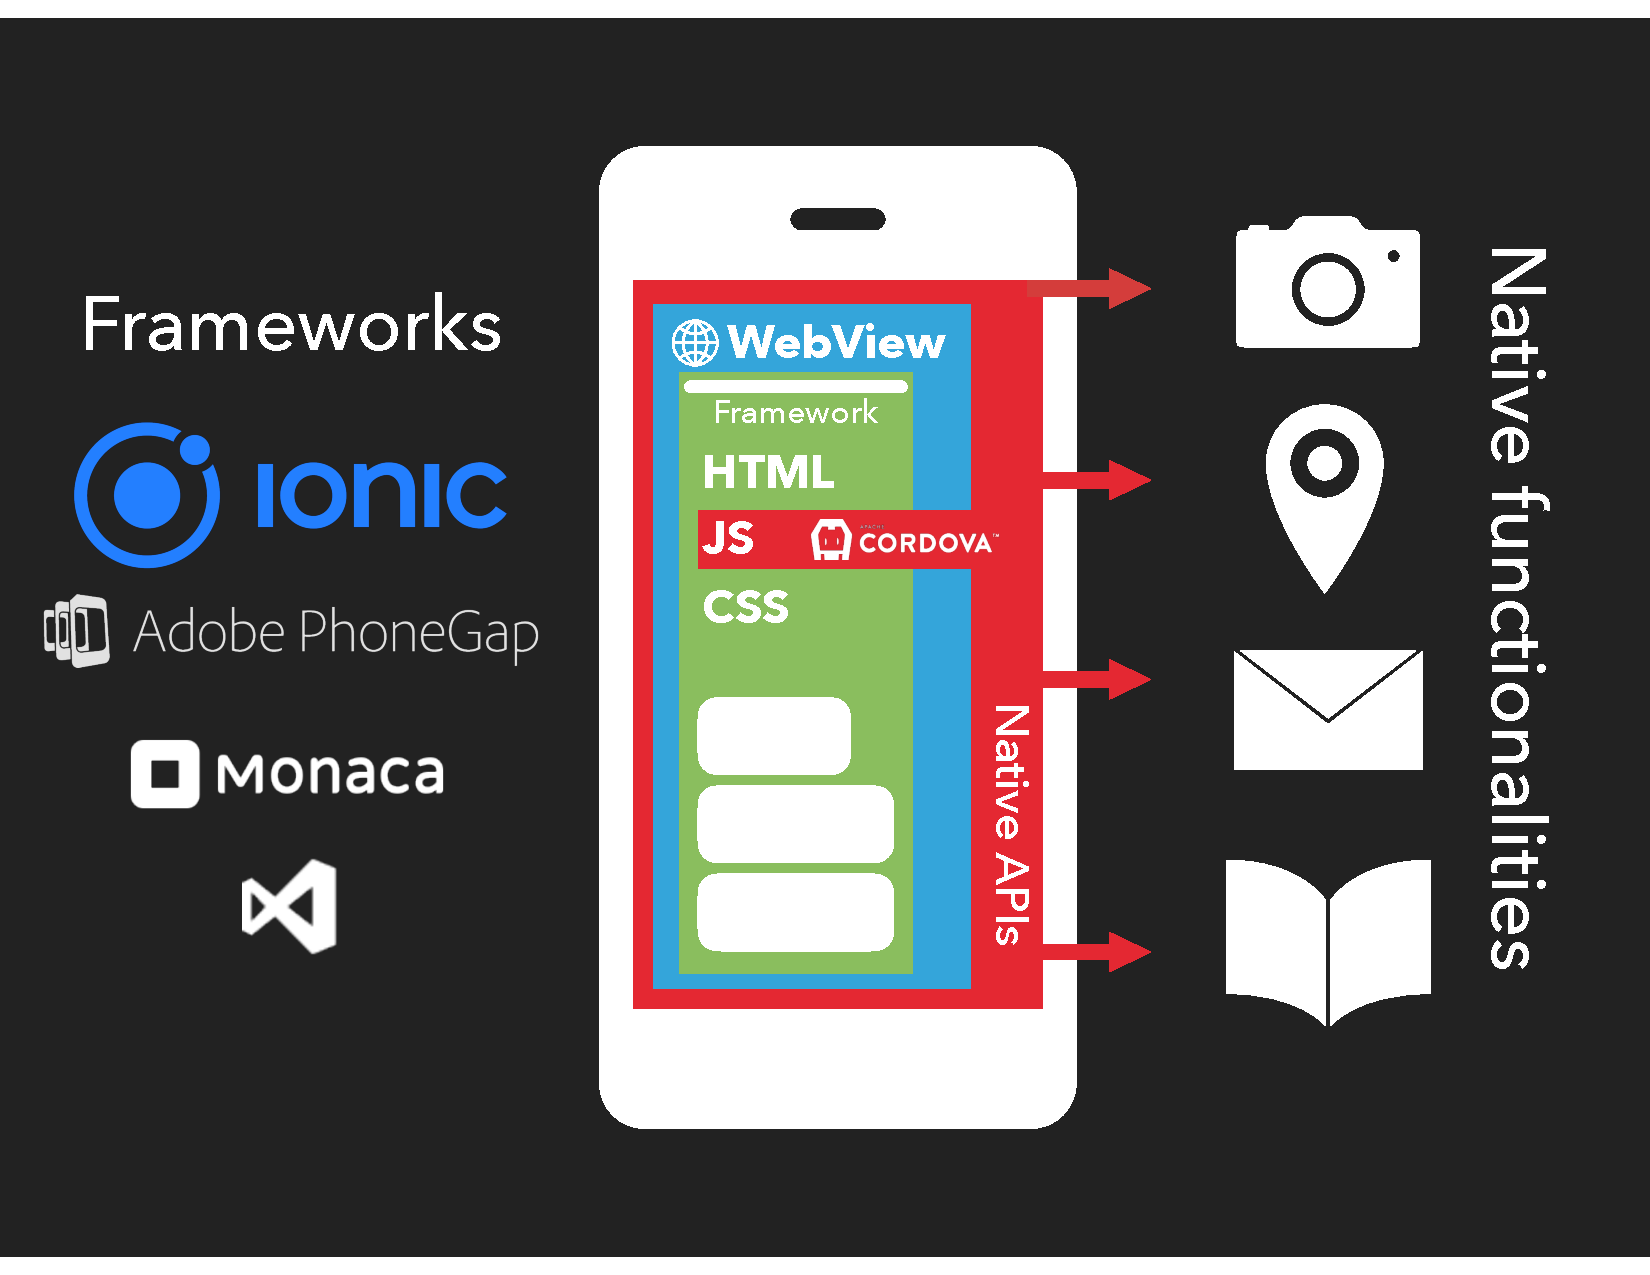
\includegraphics[width=1\textwidth]{img/hybrid.pdf}
	\vspace{-0.8cm}
	\caption{Contrary to native applications, Apache Cordova based applications contain just one activity. This activity has a basic layout with a central element: a \textit{Web view}}
	\label{hybridCordova}
\end{figure} 


Because of the differences between React Native and Apache Cordova, some argument that React Native is not hybrid. Given the fact that React Native apps can be crawled as native applications, henceforth, when we refer to hybrid applications we will refer exclusively to apps that use a Web View to present the GUI.

\subsection{Testing  hybrid applications}

Most of the research conducted in hybrid applications is focused in two categories: Debugging and Security.

\subsubsection{Debugging}

The most popular tool for debugging hybrid applications and remote web views is Chrome Developer Tools \cite{cdt}. These tools are directly built into the Google Chrome browser. Accessing to \texttt{chrome://inspect} displays the lists of web views in the devices connected through ADB. Once the browser is remotely inspecting the web view, all the errors, crashes and logs from JavaScript are printed in the computer's console. With Google Chrome, developers have access in real time to the DOM elements, network settings, and JS console to profile and audit the applications performance.

The first remote debugger was introduced in 2010: winre (WEb INspector REmote)\cite{weinre}. It was part of the Apache Cordova project, however it is being deprecated due to the increasing functionality of the Google Developer Tools. There are tools based on Google Developer Tools that enhance debugging functionality, such as the Monaca Debugger\cite{monacaDebugger} which include Cordova Plugins Supoprt and collaboration tools.


There is an approach to debug hybrid applications based on static analysis: HybriDroid\cite{7582763}.  It includes a built in bug detector based on a call graph which founds 4 types of bugs: MethodNotFound (when a JavaScript method call cannot find any target Java method to call), TypeOverloadedBridgeMethod (when JavaScript tries to use Java overloading), NotCompatibleTypeConversion (when a JavaScript type is not compatible with Java), and MethodNotExecuted (when a Java method returns an Array)\cite{7582763}.

\subsubsection{Security}

Tools and techniques related to security, are relevant to our approach because they examine the web view, and are able to analyze properties of hybrid applications.

This has been an important research topic in hybrid applications because of the possibilities of \textit{cross-language code injection}. Jin \textit{et al.} \cite{Jin:2014:CIA:2660267.2660275} define that this problem is inherited from Cross-Site scripting (XSS); additionally to their study, they developed a vulnerability detection tool.  These vulnerabilities have been detected, and numerous tools to report them have been created: NOFRAK \cite{georgiev_jana_shmatikov_2014}, Draco \cite{Tuncay:2016:DSU:2976749.2978322}, \cite{10.1007/978-3-319-27659-5_22}. Some of these approaches are based on instrumentation to  reduce the attack surface \cite{Shehab:2014:RAS:2688412.2688417}. BridgeTaint\cite{8410576} is 'a bi-directional dynamic taint tracking method that
can detect bridge security issues in hybrid apps' \cite{8410576}. It analyzes privacy leaks and code injection when the app uses bridge communication dynamically. Another tool that addresses this problem is HybriDroid\cite{7582763} which additionally to the bug detector, detects taints and leaks between Java and JavaScript. In comparison, BridgeTaint is able to detect security issues of apps built with frameworks, when HybriDroid sometimes do not.

Another topic related to security is the detection of SSL errors, Zuo  \textit{et al.} \cite{Zuo:2015:ADS:2714576.2714583} present an approach to detect statically and dynamically vulnerabilities of this kind.

\subsubsection{GUI ripping tools}

As described above, GUI ripping tools for native apps are diverse and numerous, however, as of today, there is not a single approach that focuses on GUI ripping or crawling based on hybrid applications (based on a web view). Some of the tools mentioned in section \ref{native:ripping} could work because of their implementation and the dynamic detection of components, nevertheless, they have flaws detecting different states and crashes.



 % INCLUDE: related work
\chapter{Proposed Approach}
\label{chapter3}
Before describing the proposed approach we clarify the meaning of context, domain, usage, and GUI models. A domain model describes data, entities and their relationships in an application; it looks like a network of interconnected objects, where each object represents meaningful entities and concepts. Information in a domain model is useful to determine inputs and outputs in an application under test. A graphical user interface model (GUI) is also an informative model that represents all the graphic components and views of an application, and the events that trigger transitions among the views; it is commonly represented as a state diagram and it has been widely used for GUI ripping \cite{amalfitano_fasolino_tramontana_carmine_memon_2012}. A context model \cite{crashscope} represents the surrounding conditions in which an app runs; in the case of mobile applications, it also includes sensors, networking, available hardware information (\eg device model, processor version), screen resolution and O.S version. An usage model describes how users can interact with an application and what functionalities are offered to them \cite{monkeylab}.

By augmented model (or multi-model) we mean the combination of the aforementioned models, in a single model that synthesizes relevant information.  
%A top-down approach will be used to present our approximation to augmented models for Android apps. We propose to extract a context model, a domain model a GUI model and an usage model. Our starting point is an APK and a virtual o real device. The APK can be decompiled through reverse engineering tools (\eg APK Tool \cite{apkTool}) to do static code analysis. To dynamically explore the app, we propose automated installation of the APK into a device, followed by automated exploration through ripping strategies. 
More formally, a multi-model is a directed graph. $G = (V,A)$, with
$V $ a set of states, in which each state has a unique combination of contextual variables,  GUI elements and domain entities; and 
$A$ a set of transitions, where each transition is a contextual change in the APP or an user interaction in the GUI that triggers a change in the app to a new state.

We illustrate the multi-model concept with the example presented in \figref{multimodel}; the Figure depicts an abstraction for a multi-model  generated dynamically and statically from a test app developed by the authors. The multi-model  has 3 states (\textit{S1}, \textit{S2} and \textit{S3}), and 2 edges (\textit{T1} and \textit{T2}). In this example, the app is impacted by contextual changes. %Turning off Wi-Fi in the home screen activates an alert dialog (S3) that warns the user about using bluetooth because Wi-Fi is off.  Otherwise, clicking a button in the home screen (S1) changes the app to a state where a domain element can be created by filling a text box (S2). In this scenario, a multi-model is representing a complete abstraction with domain, GUI, context and usage elements.

\begin{figure}[t]
	\centering
	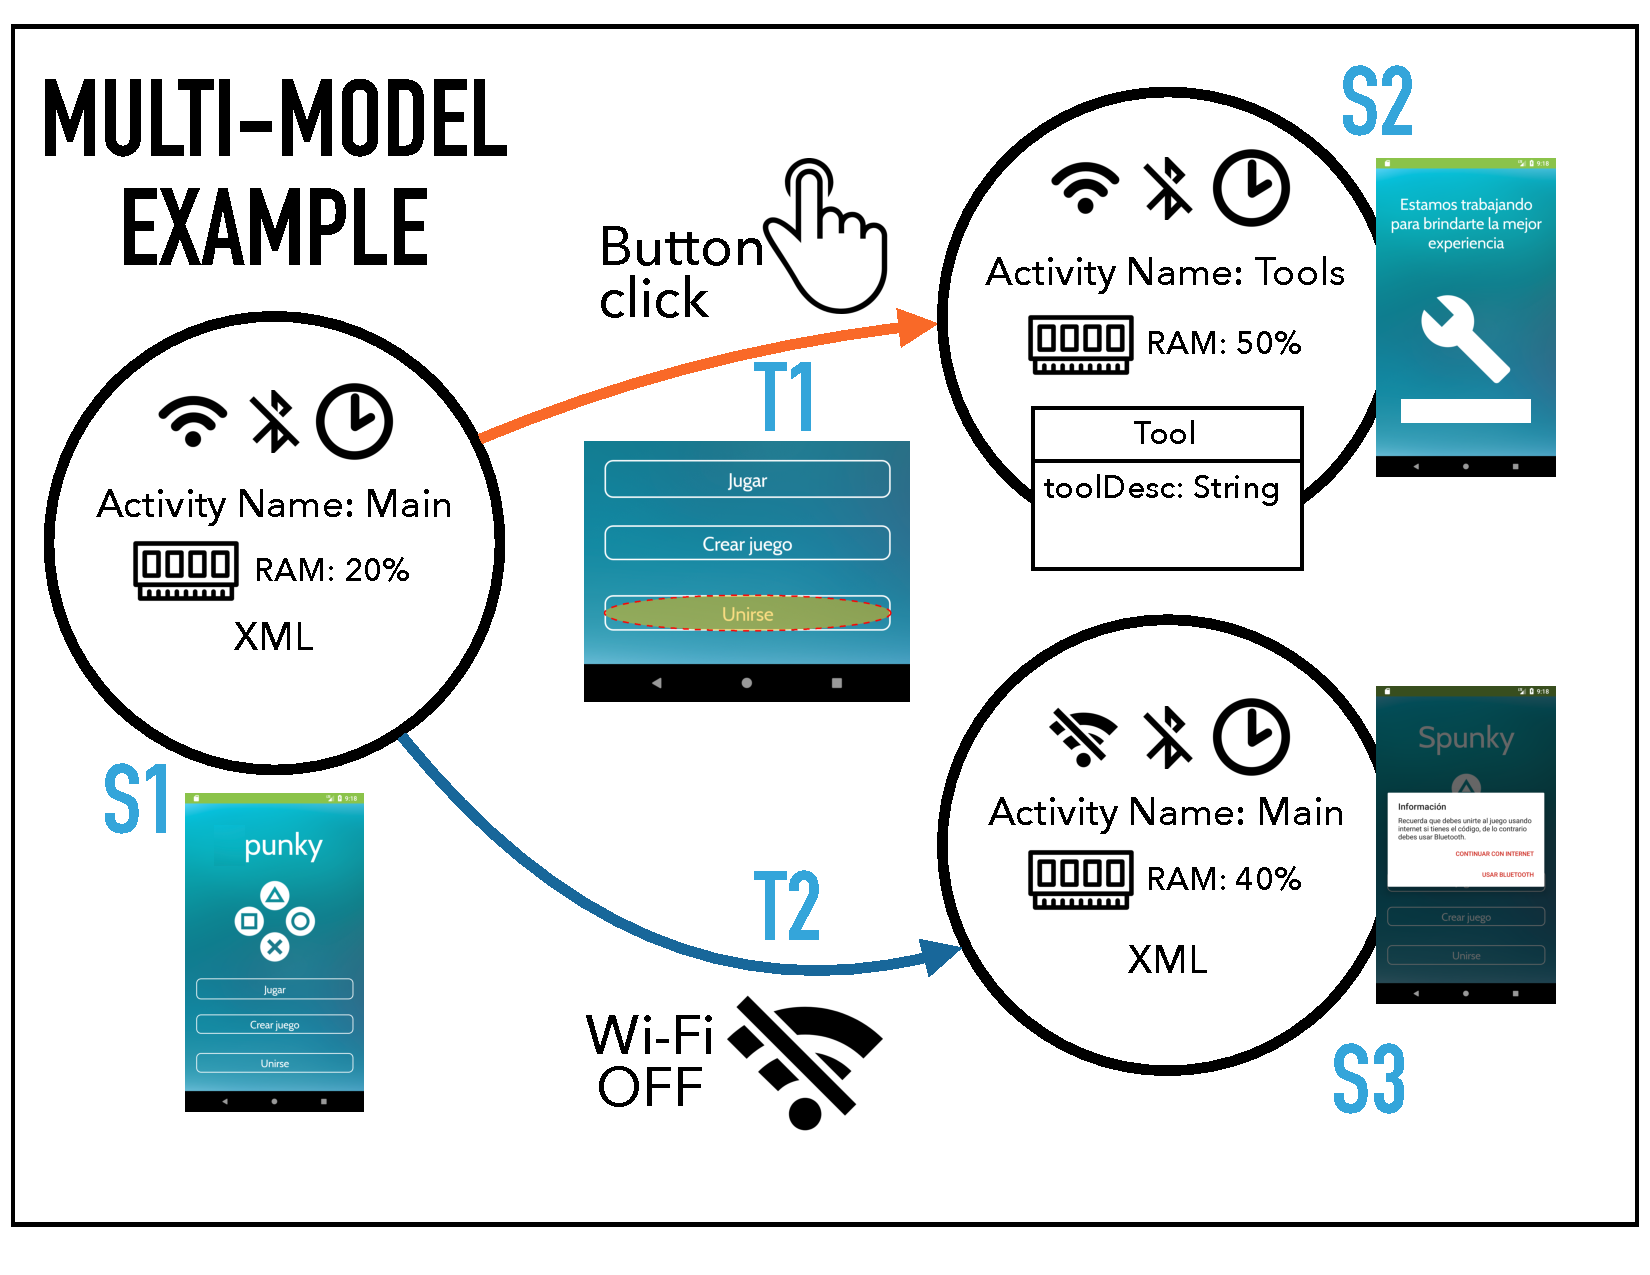
\includegraphics[width=1\textwidth]{img/multimodel.pdf}
	\vspace{-0.8cm}
	\caption{Example of multi-model generated from an Android app. The states and transitions are a subset of the complete multi-model for the analyzed app.}
	
	\label{multimodel}
\end{figure} 


\textit{S1} is the home window of the application. It is a state that mixes graphical, usage and context information. \textit{S1} occurs when Wi-Fi and cellular networks are active. On average, when this state is  active, the device has an availability of 80\% of its memory. %\textit{S1} also contains a XML screenshot of its graphical layout and an image.  
From \textit{S1}, the app flow can go to two states (\textit{S2} and \textit{S3}). The transition from \textit{S1} to \textit{S3} (\textit{T2}) occurs when Wi-Fi is turned off. \textit{S3} is a state running the same activity as \textit{S1}, however, it displays an alert message that fades out other buttons and the background. \textit{S3} is more memory greedy than the initial state.

Transition \textit{T1} changes app state from \textit{S1} to \textit{S2}. This transition is activated by clicking the button located at the bottom of the screen. Once this button is pressed, \textit{S2} is activated.  Context, graphical and usage information is also available in \textit{S2}, however, it also includes domain-related information because there is a text-input for collecting information from the user; thus, we consider the activity (\ie the Android window related to \textit{S2}) as an entity named ``Tool” with a string field called ``toolDesc”.

%Summarizing \figref{multimodel}, this example app with 3 states is affected by contextual changes. Turning off Wi-Fi in the home screen activates an alert dialog. When this alert appears, more RAM memory is being used in the device. Clicking a button in the home screen changes te app to a state where a domain element is created by filling a text box. In this scenario, a multi-model is representing a complete abstraction with domain, GUI, context and usage elements.

\section{General Approach}

\begin{figure}[t]
	\centering
	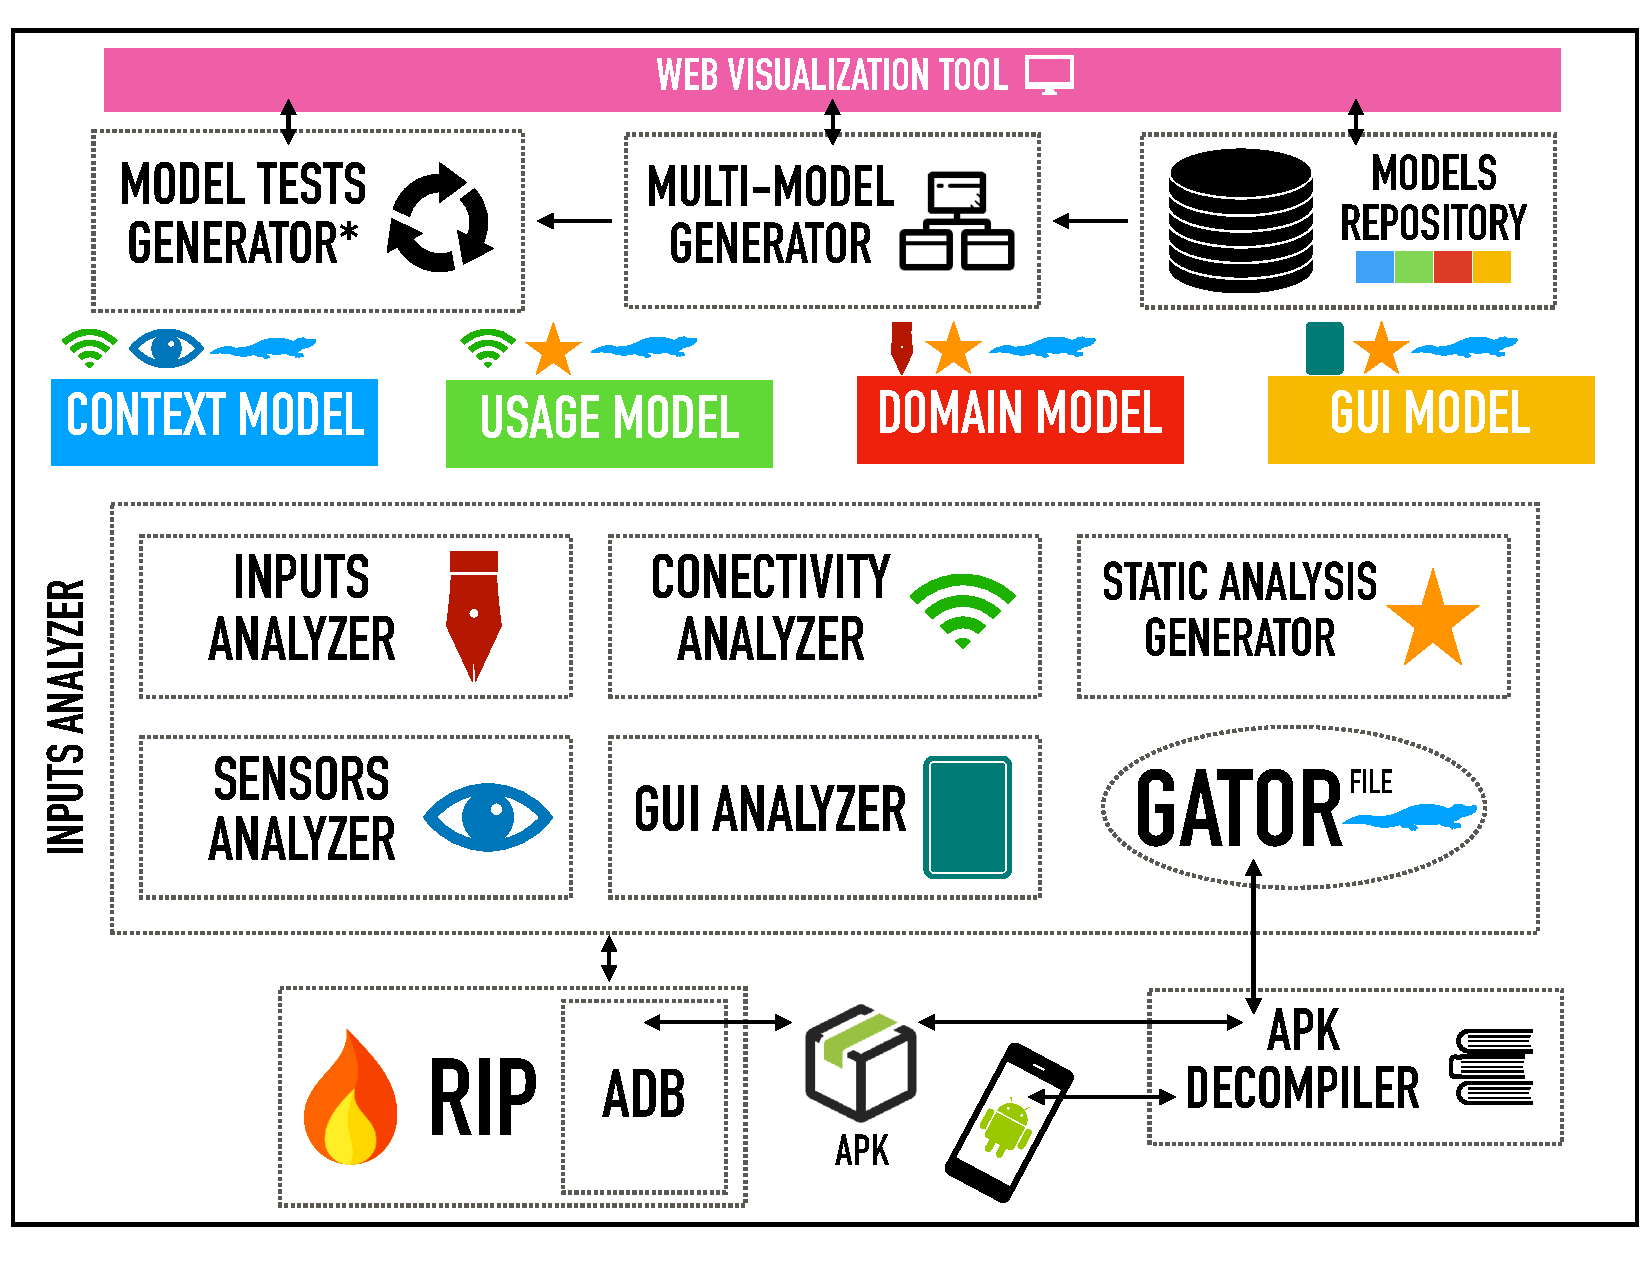
\includegraphics[width=1\textwidth]{img/generalArchitecture.pdf}
	\vspace{-0.8cm}
	\caption{Proposed architecture (\textbf{RIP}) for extracting augmented models for Android apps.}
	\label{generalArchitecture}
\end{figure}	

We have designed an  architecture \figref{generalArchitecture} that enables a series of stages that include: ripping, automatic extraction of static and dynamic models, generation of multi-models and model-based tests generation.

The multi-model generation starts by ripping the app under test. For this purpose, we have designed and developed a desktop tool called \textbf{RIP}, which is publicly available at \url{https://github.com/TheSoftwareDesignLab/rip}. It is an automation software that executes a series of actions and emulates user interactions into an Android device to extract models; this is done through the Android Debug Bridge (ADB) \cite{adb}, a command-line tool that provides access to an Android device over USB or Wi-Fi. In comparison to monkey/random testing tools that generate random interactions to find bugs and corner cases, \textbf{RIP} follows an strategy to explore the application based on the dynamic content that appears on a device screen (like other rippers do). \textbf{RIP} not only simulates user interactions in the screen; \textbf{RIP} also executes contextual changes to the application that vary the network configuration and the readings of the sensors (\eg accelerometer, gravity, gyroscope, light, proximity, magnetic field).  During the execution,  \textbf{RIP} collects GUI-related, domain-related. sensors-related, and resources-related information. In addition, screenshots and  GUI-hierarchies are collected for each state.

Our approach differs from existing ones because we are able to (i) generate a comprehensive list of contextual changes, (ii) extract a domain model from GUI states,  (iii) augment the dynamically-generated model with information collected statically, and (iv) considers exploration of hybrid applications. Due to security restrictions imposed by Android devices and the Android framework, in order to enable contextual events execution via ADB (\eg airplane mode, Wi-Fi), it is necessary to run the commands in a rooted physical device or an emulator.

\textbf{RIP} takes advantage of static code analysis to enrich the final generated model. When the ripping process finishes, RIP augments the collected model with a graph generated statically by GATOR \cite{gator}, a static reference analyzer tool for GUI objects in Android. This tool has been chosen because its context-aware approach in static code analysis \cite{yang_yan_wu_wang_rountev_2015}. GATOR finds static references to GUI components and determines its control flow. If \textbf{RIP} identifies missing states (\ie states detected by GATOR but not by \textbf{RIP}), it adds the new states to the dynamically generated model. Thus, the  GUI and usage models are represented by the combination of transitions and states information extracted from the ripping and GATOR.

GATOR code is not included in \textbf{RIP}. To combine static information with RIP's execution, GATOR analysis should be run first, and then passed to \textbf{RIP}. An example of the file that \textbf{RIP} imports from GATOR is presented in the code example \ref{gatorFile}

\begin{lstlisting}[language=json, caption={Fragment of a GATOR file obtained from a native application}, label={gatorFile}, firstnumber=1]
{ "nodes": [{
"id": 2160,
"name": "com.simplemobiletools.commons.activities.FAQActivity"
}, {
"id": 2076,
"name": "android.view.Menu"
}, {
"id": 2140,
"name": "android.view.Menu"
}, {
"id": 14106,
"name": "android.app.DatePickerDialog"
}],
"edges": [{
"source": 2076,
"target": 2140,
"event": "implicit_power_event"
}, {
"source": 14106,
"target": 14106,
"event": "implicit_home_event"
}, {
"source": 2140,
"target": 2140,
"event": "implicit_rotate_event"
}, {
"source": 2160,
"target": 2160,
"event": "implicit_home_event"
}]}
\end{lstlisting}

\section{RIP components}		

Our architecture defines a layer of analyzers that guide \textbf{RIP} during the models extraction:

\subsection{GUI analyzer}

It extracts the hierarchy of graphical components in the app. It is able to differentiate app GUI states based on the analysis of the GUI hierarchy represented as an XML file. It means, the construction of the GUI model is done iteratively, according to the app exploration. To determine if two views are different, a decision process is followed. Firstly, if the activity names differ from each other, the two views are classified as different states. Otherwise, if the activity names are the same, then the XML is analyzed; each view is compared by the number of elements, checked boxes,  buttons, labels content, alerts, and messages.  In the case of menus or dialogs that are displayed on a view, we consider them also as states.

\begin{lstlisting}[language=xml, caption={XML dump from an app, containing the layout hierarchy},label={xmlDump}]
<?xml version='1.0' encoding='UTF-8' standalone='yes' ?>
<hierarchy rotation="0">
<node index="0" text="" resource-id="" class="android.widget.FrameLayout" package="com.clockwork.mcdonalds"
content-desc="" checkable="false" checked="false" clickable="false" enabled="true" focusable="false" focused="false"
scrollable="false" long-clickable="false" password="false" selected="false" bounds="[0,0][1080,1794]">
<node index="0" text="" resource-id="" class="android.widget.LinearLayout" package="com.clockwork.mcdonalds"
content-desc="" checkable="false" checked="false" clickable="false" enabled="true" focusable="false"
focused="false" scrollable="false" long-clickable="false" password="false" selected="false" bounds="[0,0][1080,1794]">
<node index="0" text="" resource-id="android:id/content" class="android.widget.FrameLayout" package="com.clockwork.mcdonalds"
content-desc="" checkable="false" checked="false" clickable="false" enabled="true" focusable="false"
focused="false" scrollable="false" long-clickable="false" password="false" selected="false" bounds="[0,63][1080,1794]">
<node index="0" text="" resource-id="" class="android.widget.ImageView" package="com.clockwork.mcdonalds"
content-desc="" checkable="false" checked="false" clickable="false" enabled="true" focusable="false"
focused="false" scrollable="false" long-clickable="false" password="false" selected="false" bounds="[0,63][1080,1794]" />
</node>
</node>
<node index="1" text="" resource-id="android:id/statusBarBackground" class="android.view.View" package="com.clockwork.mcdonalds"
content-desc="" checkable="false" checked="false" clickable="false" enabled="true" focusable="false"
focused="false" scrollable="false" long-clickable="false" password="false" selected="false" bounds="[0,0][1080,63]" />
</node>
</hierarchy>
\end{lstlisting}

%Some thresholds can be configured by the developer to change the sensitivity of states detection. 

The set of states gathered from visual information are the source for the GUI model. \textbf{RIP} captures image screen-shots and  XML layouts from every state it has found. It also records the interaction/event that triggered the state transition (\eg pressing a button); note that state transitions are modeled as edges connecting states. To extract the XML layout information, \textbf{RIP} executes the command \verb|adb shell uiautomator dump|. Eventually, the device stores this dump into an XML file such as the code example \ref{xmlDump}. Because this file is stored in the SD card, it must be extracted and parsed in the host computer. To capture the image snapshot of the device, a remote screen-shot is invoked with the command \verb|adb shell screencap|. All the files in the devices are extracted through \verb|adb pull|.

%The GUI model finally will be shown as a state diagram, including transition as edges connecting different states of the application.


\subsection{Inputs analyzer}

It enables \textbf{RIP} to identify user input-related GUI Android components and interact with them accordingly (\eg check boxes, text boxes, lists, scrollable views).  \textbf{RIP} creates random input data for the components based on the input types defined for text fields, and the component nature (\eg a check box can be activated or deactivated). Keyboards that appear on the screen and GUI components meta-data, give us clues about concepts and domain entities that are part of the domain model of the application. 
We define entities of the domain model as views that have input elements. Each entity has a set of attributes that correspond to input-related components in the view, and the attributes type is inferred from the type of input allowed (\eg numbers, special characters, boolean check, lists, \etc). 

\subsection{Sensors analyzer}

During the ripping, \textbf{RIP}  turns off/on sensors, randomly. The sensors analyzer identifies which sensors the application has access to from the app's manifest file. Once the sensors analyzer has this information, it detects the states where sensors are on and off using specific ADB commands. 

To obtain a detailed list of sensors, \textbf{RIP} invokes the command \texttt {adb shell pm list features}. The available sensors in the device are listed as features (\eg \verb|hardware.camera|,  \verb|hardware.sensor.gyroscope|, \verb|hardware.sensor.light|)

\subsection{Connectivity analyzer}

This component identifies connectivity status of the app during all the ripping execution. Once the GUI has detected an initial set of states, it sends requests to the device in order to control Bluetooth, Wi-Fi, celullar networks and airplane mode. \textbf{RIP} triggers connectivity changes in every view of the application. If an error occurs or the GUI changes after the contextual change, then a new state is  discovered and added to the model.

To determine the connectivity settings of the device, \textbf{RIP} calls the command \texttt {adb shell dumpsys wifi | grep 'Wi-Fi is'} to determine Wi-Fi status, \texttt {adb shell dumpsys wifi | grep 'mAirplaneModeOn'} to determine Airplane Mode, etc. The activation or deactivation of these settings is done with the commands  \texttt {adb shell svc wifi (disable|enable)}, \texttt {adb shell svc bluetooth (disable|enable)}, \texttt {adb shell svc data (disable|enable)}, etc. Commands that enable or disable connectivity settings of the device require root privileges.


\subsection{Static analyzer and GATOR}
Different from the other components, it imports a flow graph of the app based strictly on static analysis, by relying on the GATOR tool \cite{gator}. GATOR creates a window transition graph with activities, dialogs and menus. The transitions of the graphs include events such as button pressings and window stack operations (push and pop). This flow graph is used to augment the model collected dynamically by  \textbf{RIP}, in particular to have a more comprehensive list of transitions and states. This graph is presented in the code example \ref{gatorFile}.

%	\begin{figure}[h]
%		\centering
%		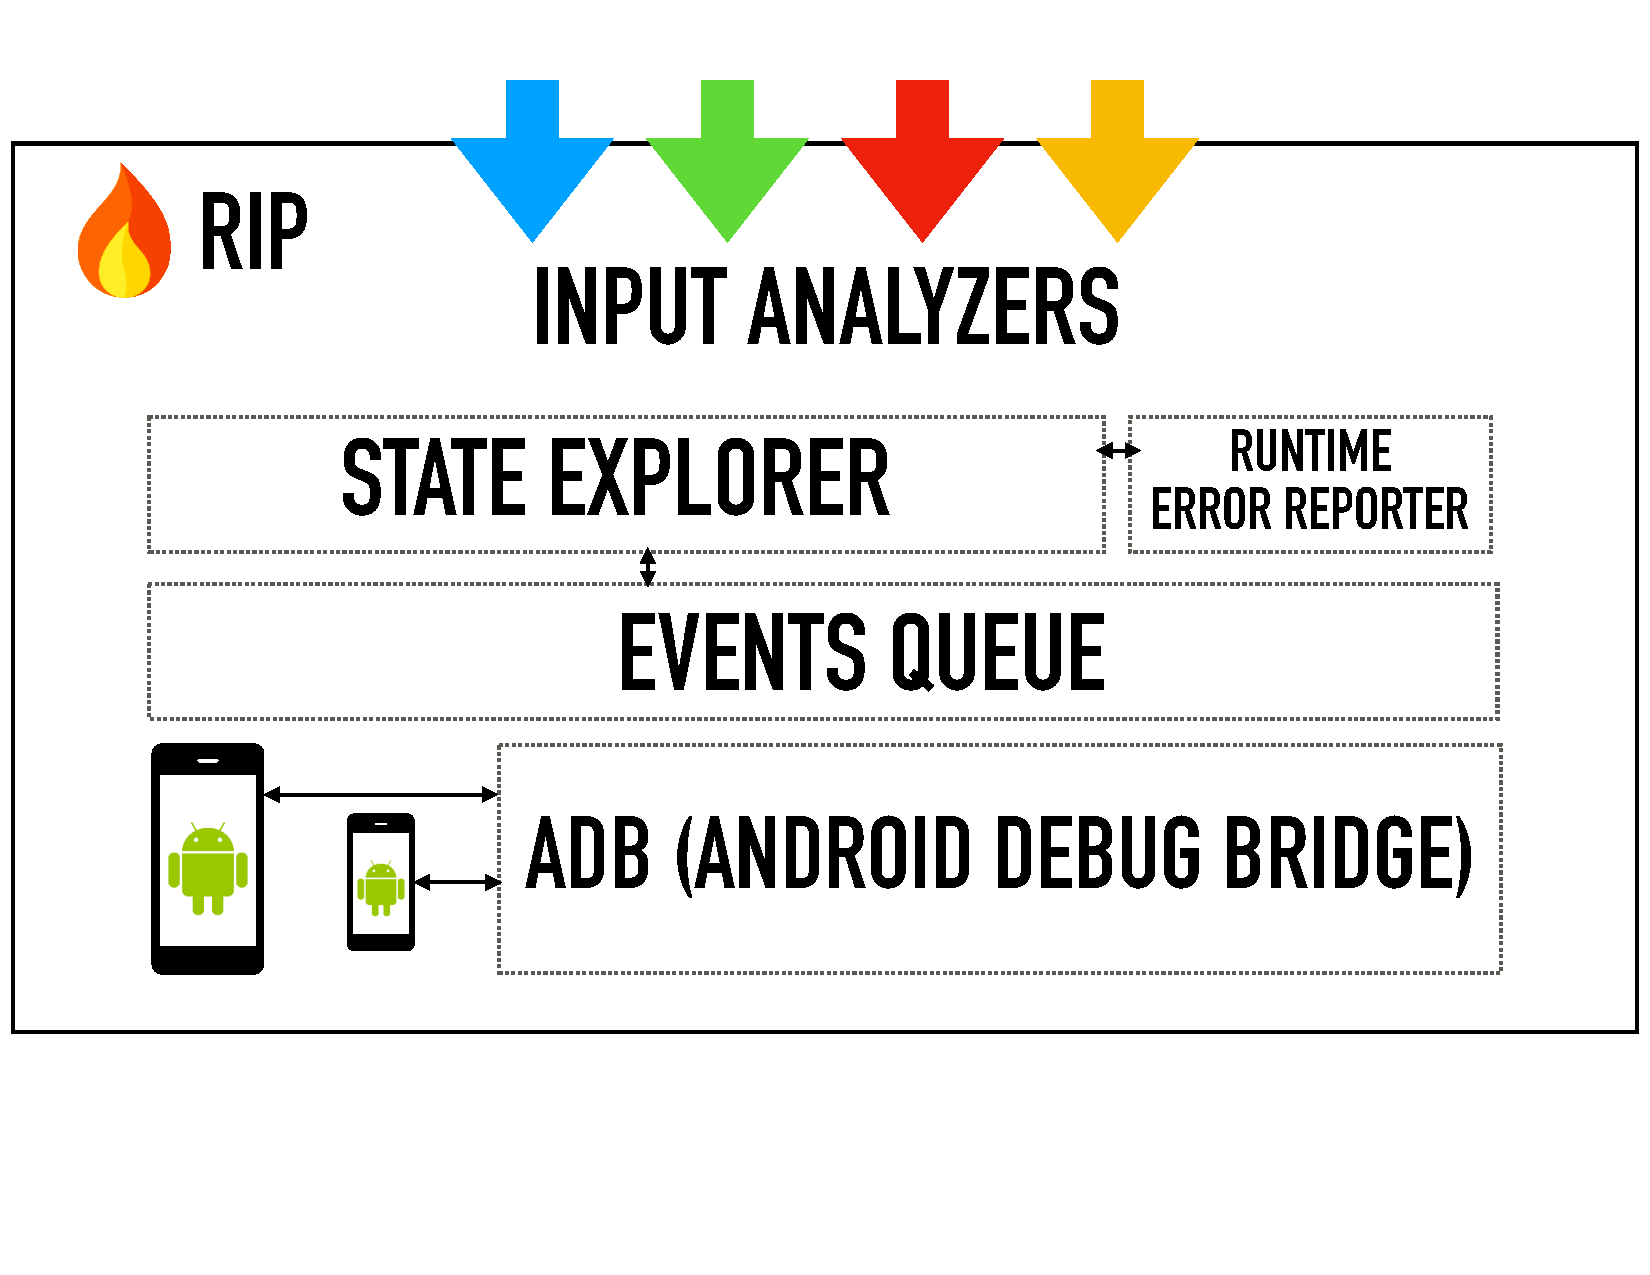
\includegraphics[width=0.5\textwidth]{img/ripArchitecture.pdf}
%		\caption{RIP components.}
%		\label{ripArchitecture}
%	\end{figure} 
%	

\subsection {RIP GUI}
It interacts directly with ADB to explore the applications dynamically and coordinates the execution of the other components. The \textbf{RIP} GUI combines the ripping, interactive data collection, and static analysis, to generate individual models and a multi-model like the one presented in \figref{real}; the \textbf{RIP} GUI also generates the model as a JSON file that can be analyzed by any other tool.

%\textbf{RIP} identifies native graphical Android elements to explore systematically every possible view of the app. This tool is able to simulate user interactions and contextual changes. RIP sends the gathered information to all the analyzers in order to build the mentioned models. \figref{real} presents a multi-model generated from our test app.

\begin{figure}[t]
	\centering
	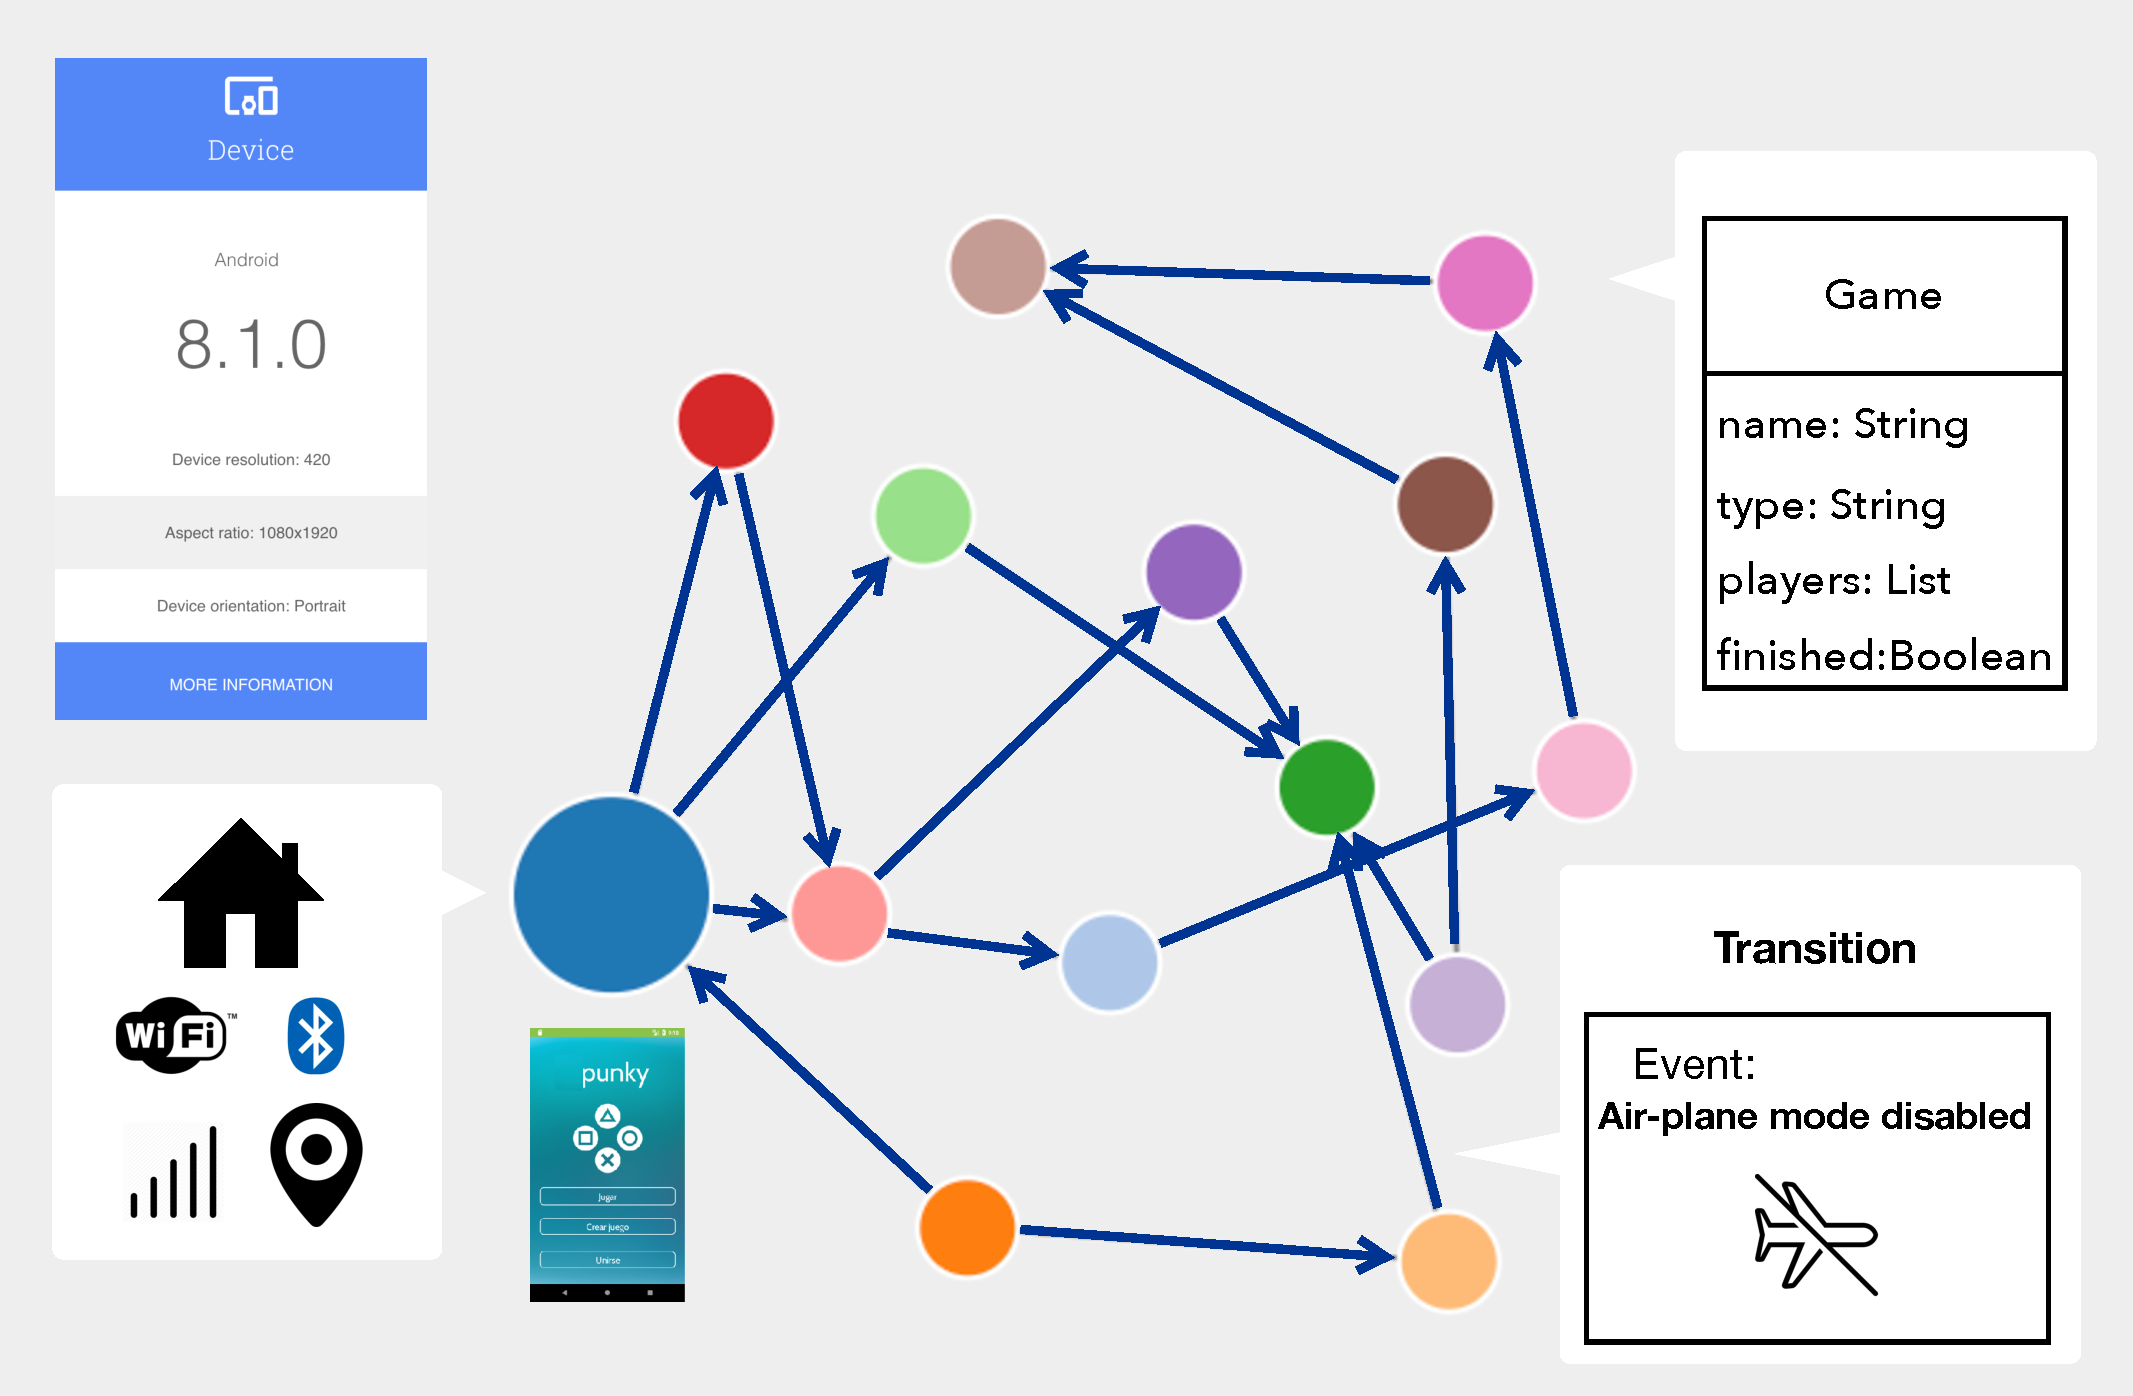
\includegraphics[width=1\textwidth]{img/multimodel-real.pdf}
	\vspace{-0.8cm}
	\caption{Example of multi-model created by RIP.}
	\label{real}
\end{figure} 

%	RIP general architecture is presented in \figref{ripArchitecture}. RIP communication with the device is done through Android Debug Bridge (ADB).
%	
%	\subsubsection{Events Queue}
%	RIP has an events queue that manages and synchronizes events between ADB and the state explorer. 
%	
%	\subsubsection{State explorer}
%	The states explorer is the controller of the automated interactions against an application. Once an APK is installed in a device, it defines the exploration strategy that RIP will follow. Input analyzers send request to the state explorer to push and pull information from the headset.
%	
%	Exploration could follow two principles. First, random exploration introduces random interactions into the app. These interactions include GUI analyzer interactions (\eg pressing random buttons, selecting check boxes, swiping), Input analyzer interactions(\eg Introducing text strings, numbers), connectivity interactions (\eg enable airplane mode, disable Bluetooth) and sensors interactions (\eg simulate a move of the accelerometer). This exploration method can be executed until a number of interactions have been done or until a timer ends.
%	
%	Second principle of exploration is guided exploration. It includes the same interactions, but this time it sets itself the objective of explore and cover the maximum amount of possible states. This kind of exploration is done by DFS and request the analyzers to create all the possible configurations for each view changing connectivity and sensors informations.
%	
%	\subsection{ Models repository}
%	
%	Models repository condenses all the generated models to be processed by the multi-model generator.
%	
%	\subsection{Multi-model generator}
%	
%	The multi-model generator takes as input the context, usage, domain and GUI models and combines all the models into a richer sate diagram.
%	
%	%\subsection{Test generator}
%	
%	%Test generator is currently not developed, however, it is a future step that will enable model-based testing based on the multi-model generation.
%	
%    \subsection{WEB visualization tool}
%    
%    Finally, a web visualization tool based on Javascript, HTML and D3 presents the final  multi-model. All the intermediate models are also included. This tools is presented in \figref{webTool}.
%    
%    \begin{figure}[h]
%    	\centering
%    	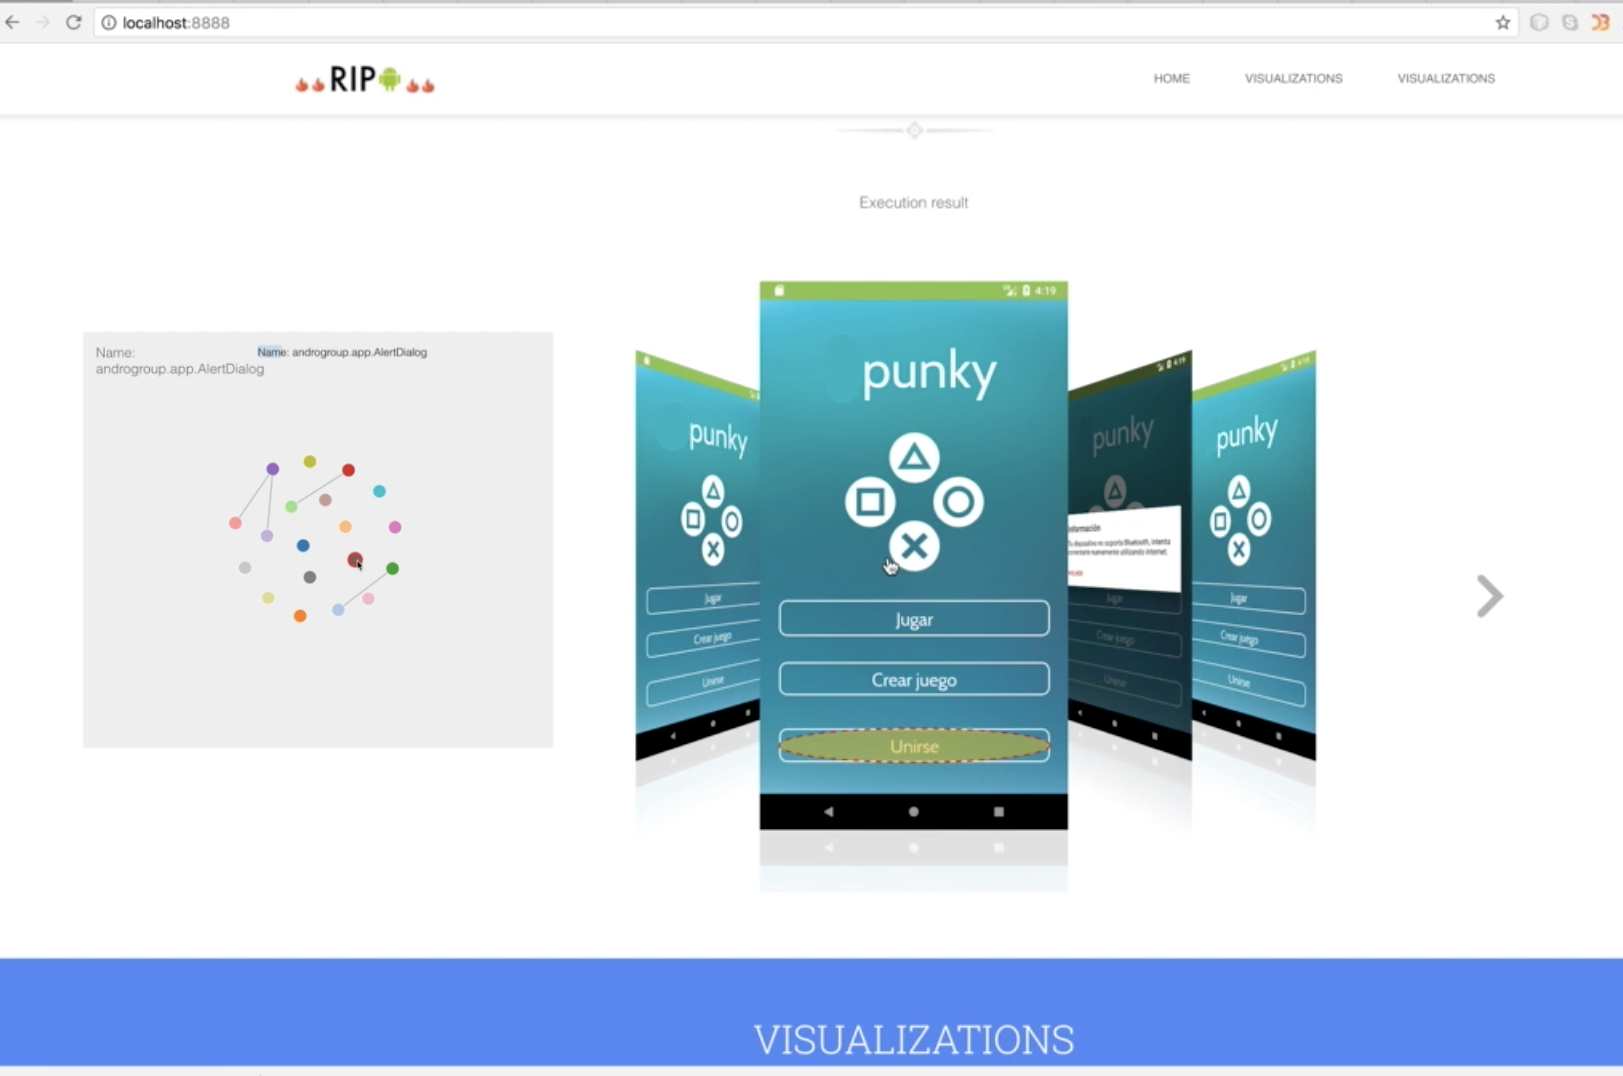
\includegraphics[width=0.5\textwidth]{img/webTool.png}
%    	\caption{WEB visualization tool}
%    	\label{webTool}
%    \end{figure} 

\section{Ripping  hybrid applications}
As described before, hybrid apps are those in which developers write significant portions of their application in cross-platform web technologies, while maintaining direct access to native APIs when required \cite{ibmHybrid}. This way of developing applications is gaining popularity among the mobile developers community because:
\begin{itemize}
	\item Reduces the time to develop cross platform apps
	\item It is based on Web technologies, which allows developers to recycle modules and components from existing Web developments
	\item Browser engines are becoming faster and mobile devices more powerful
	\item Performance differences between native and web technologies are becoming imperceptible
\end{itemize}

Currently, Apache Cordova is the component that enables the access to native iOS and Android APIs from the JS code. This piece of software gives access to Local Storage, Camera, GPS, and all the available sensors of each platform. Apache Cordova is the core of many popular hybrid frameworks such as Ionic, Adobe Phonegap, Monaca or Visual Studio. 

\subsection{Barriers for ripping hybrid apps }
Ripping native apps is different from ripping hybrid apps. The main reason is the underlying techonologies; in native apps the GUI is rendered by the view system and window manager of the  framework, in hybrid apps the GUI and events are managed by a Web View. In native applications, a native layout defines the structure of the user interface. An activity contains a hierarchy of containers and graphical objects called \textit{Views} and \textit{View groups}. These objects are also known as \textit{widgets}. Widgets could be instanced as elements such as buttons, labels, text fields, among others. View groups provide the structure of widgets and other view groups in the screen \cite{layouts}. To crawl dynamically apps, this hierarchy must be extracted continuously, and based on the layout information, the ripper can execute commands and simulate user interactions.

Contrary to native applications, most hybrid applications contain just one activity. This activity has a basic layout with a central element: a \textit{Web view} \cite{webView}. Web views are widgets that can render web content \figref{hybridCordova}. When the user interacts with elements of the web view, the JavaScript engine is in charge of changing the view. All the application logic is entirely written in JavaScript, therefore, errors, bugs and crashes are only visible to the web console. Additionally, the HTML DOM is not visible through the \verb|adb dumpsys| command.

\subsection{Strategies for ripping hybrid apps }
In \textbf{RIP}, we have defined and implemented a series of strategies designed to tackle the ripping of hybrid apps. Specifically, we consider important to maximize the coverage of states discovered and enable detection of crashes, while maintaining the  strategy of multi-model extraction and contextual exploration. 

\subsubsection{Detecting crashes in hybrid apps}
Crashes are usually the result of uncaught exceptions. Other crashes come from ANRs (\textit{Application Not Responding}), permission denials, network errors, and bad practices. These kind of crashes are well defined in the Android Developers Documentation and if one of them occurs, it is reported in the device. When one of these crashes is thrown, rippers of native apps are able to recognize them because the device writes them in the device log (logcat). In general, hybrid applications do not deal with these errors as native applications do, because their errors  are written in the JS console. In order to capture errors in hybrid applications, RIP reads continuously the WebView console with the help of Chromium.

While \textbf{RIP} crawls a hybrid application, it listens to the web console, and stores the web errors associated with each state. As these errors occur in an embedded web browser, all the HTTP errors can be associated to the running application. %As an example, in Figure \ref{hybridError} is depicted a 503 HTTP status code: Service unavailable.

\subsubsection{Maximize the coverage of states discovered}
In order to maximize the coverage of states discovered, \textbf{RIP} must interact with every 'clickable' element inside the web view. The exploration should not be focused on finding and interacting with Android widgets, but with every new component accessible in the web view. A better approximation to explore the hybrid GUI should extract and parse the DOM of the web components with the help of the Chrome inspector, however, this is considered as future work.

We found experimentally that introducing some randomness to the ripping process in these applications improves the discovering of new states, because not all the web elements can be extracted solely with UIAutomator, and always remains actions of the application that could not be accessed systematically.

Finally, a key step that improves exploration of hybrid apps is triggering contextual changes, specifically, toggling network and Internet settings. This occurs because sometimes, all the web view content is not served just from the mobile device, but also from external servers in the Internet. Hybrid applications are highly prone to errors due to contextual changes.

\begin{lstlisting}[caption={Pseudocode describing the Ripping process},label={pseudocode}]
transitions = []
discoveredStates = []
contextualChanges = [rotateScreen, turnOnWifi, ...]
func explore(t):
	s.clickOrExecute()
	transitions.push(s)
	if thisIsANewState():
		discoveredStates.push(currentState)
	if state.hasClickableElementsLeft():
 		for everyClickableElementInState c:
     		if c has not been clicked:
         		explore(c)
 	elif !state.hasClickableElementsLeft() and !state.contextualChangesDone():
 		for every cc in contextualChanges:
 			explore(cc)
 	elif state.ContextualChangesDone()
 		if state.isHybrid():
 		 	enableJSConsole()
 			action = randomAcctions()
 			explore(action)

\end{lstlisting}

	% INCLUDE: system
% !TEX root = ../thesis-example.tex
%
\chapter{Conclusion}
\label{chapter5}

The results from our empirical study suggest that  automatically extracting augmented models from Android apps enables better understanding of the apps. For modern mobile applications, ripping apps --- but based only on GUI exploration--- is not enough because they are context-aware. To that end, context, GUI, usage and domain models should be extracted and combined together to build more useful and comprehensive augmented models.

Still performance of \textbf{RIP} exploring native applications is lower than existing baseline tools' (based only on GUI ripping), however enabling contextual changes in exploration allows \textbf{RIP} to find states that these tools are not able to detect. 

Our tool bridges the gap of ripping hybrid apps, and it is the first approach that focuses in exploring dynamically these applications. \textbf{RIP} outperforms industry and academy state of the art tools in the exploration of hybrid apps.

\textbf{RIP} is able to detect WEB and HTTP crashes from native hybrid applications based on the WebView Javascript console whereas native based rippers only detect crashes such as \texttt{IOException} or \texttt{OutOfMemoryError}. This combination of web information and native informations gives \textbf{RIP} and advantage over other existing tools.

The future of mobile application development is uncertain, however, in the short and medium term hybrid applications will start growing faster because of the advances in web technologies, the substantial improvement in the performance of today's mobile devices and the cost reductions of building cross-platform applications with a single language, a single UI and a single technology.

 To summarize, the objectives of the thesis were accomplished: an approach for improving automated testing of mobile apps has been developed and integrated into a new tool called \textbf{RIP}; a software that extracts multi-models, and performs rip-based crash detection. The performance of this tool has been evaluated and compared, finding its multi-model exploration and ripping capabilities in hybrid apps its main strengths.

\section{Future work}

There is a lot of work to be done regarding tests and experiments, improving our tool and expanding \textbf{RIP} to new horizons in mobile software testing.

\begin{itemize}
	\item Introduce more applications and tools in the empirical study could gives us a better understanding of the possible improvements to RIP and our augmented-model extraction strategy.
	
	\item Further studies will be conducted to evaluate and improve automated exploration of the apps, comparing states discovered by our approach against states discovered by users' interactions.
	
	\item Improve the GUI ripping algorithm in \textbf{RIP} for native apps. \textbf{RIP} state discovery strategy based only on the GUI model is below tools like \textit{DroidBot} and \textit{Firebase Test Lab Robo Test}. Improving the ripping strategy in this case, will increment the coverage of states discovered during multi-model ripping.
	
	\item Convert \textbf{RIP} into a cloud based service. \textit{Firebase Test Lab Robo Test} showed us the benefits of running automated tests in the cloud, freeing testers from manual tasks, enabling parallel execution, and making it more accessible and easy to use.
	
	\item Integrate \textbf{RIP} with Google Chrome Dev Tools, to analyze hybrid applications DOM without restrictions and inspect more information for these applications.
	
	\item Analyze accessibility issues in Android applications based on RIP's state discovery approach. Accessibility services could be discovered and tested to make apps more useful and accessible for everyone.
	
	\item In this document, we propose to take advantage of the augmented models and implement multi-model-based testing. Augmented models contain much more information than traditional state diagrams of GUIs. All things considered, multi-models have richer information that will enable generation of more effective test suites. The proposed multi-model could be used to generate test cases, first, using the context variables to define the environmental conditions of the test cases; secondly, generating  inputs in test cases by relying on domain entities and attributes; finally, using the GUI and usage information to provide test cases based on developer requirements, such as coverage or specific functionalities. Model based testing strategies could be able to generated rich test suites, containing all the information from the augmented model. 
	
\end{itemize}


 % INCLUDE: conclusion
\cleardoublepage

\printbibliography
\cleardoublepage

\listoffigures
\clearpage

\listoftables
\clearpage

% !TEX root = ../thesis-example.tex
%
\pagestyle{empty}
\hfill
\vfill
\pdfbookmark[0]{Colophon}{Colophon}
\section*{Colophon}

This thesis was typeset with \LaTeXe. It uses the \textit{Clean Thesis} style developed by Ricardo Langner.
Firebase is a trademark of Google LLC.
%\cleardoublepage
%% !TEX root = ../thesis-example.tex
%
%************************************************
% Declaration
%************************************************
\pdfbookmark[0]{Declaration}{Declaration}
\chapter*{Declaration}
\label{sec:declaration}
\thispagestyle{empty}

You can put your declaration here, to declare that you have completed your work solely and only with the help of the references you mentioned.

\bigskip

\noindent\textit{\thesisUniversityCity, \thesisDate}

\smallskip

\begin{flushright}
	\begin{minipage}{5cm}
		\rule{\textwidth}{1pt}
		\centering\thesisName
	\end{minipage}
\end{flushright}

%*****************************************
%*****************************************

\clearpage
\newpage
\mbox{}

% **************************************************
% End of Document CONTENT
% **************************************************
\end{document}
